\section{Choosing the Shortest Paths}
\label{sec:SP}

The described strategies (except for \emph{baseline}) may suffer from a poor choice of the initial shortest path for each agent. See the example in Figure~\ref{fig:p_counterexample}. The blue agent has two possible shortest paths. If the algorithm by random chooses the blue path, none of the sophisticated strategies can solve the relaxed instance in the first solver call. \emph{Makespan-add} would find a suboptimal solution with makespan $LB+2$, \emph{prune-and-cut} would require to increase $k$ two times to be able to use the black path, and \emph{combined} strategy would also find a suboptimal solution with makespan $LB+2$.

This issue can be mitigated by including all of the vertices on all of the possible shortest paths into the $Gres_{k}$, however, this goes against the logic of the motivational example in Figure~\ref{fig:diagonal_example}, therefore we will try to identify approaches to choose more than just one of the shortest paths to help the strategies.

Since the choice of the shortest paths acts as a preprocessing stage, we aim for fast heuristic techniques. For this reason, each agent is treated individually, without considering the interference with shortest paths of the other agents. We propose the following four sensible approaches to pick which vertices should be included in the initial restricted graph $Gres_{0}$. All of the described strategies, then, work the same as was described in the previous section.

\begin{figure*}[ht]
\centering

\begin{subfigure}[t]{0.99\columnwidth}
\centering
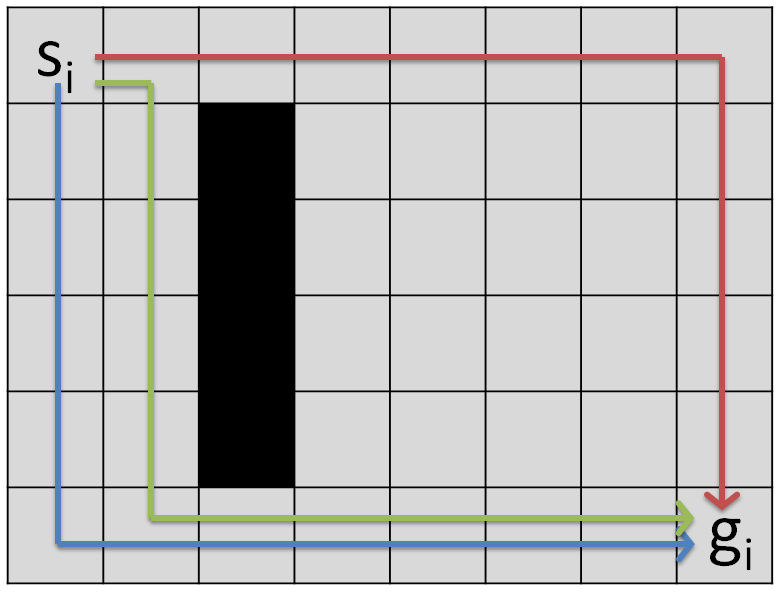
\includegraphics[width=0.45\columnwidth]{img/distant_wrong.PNG}
\caption{The greedy approach starting at $s_i$ chooses an undesirable green path due to the fact that it tries to make the path most divers (to the previously planned blue and red paths) from the start without the knowledge of the rest of the map.} %After passing the obstacle, the approach is forced to choose the same vertices as are on the blue path.}
\label{fig:distant_wrong}
\end{subfigure}
\hfill
\begin{subfigure}[t]{0.99\columnwidth}
\centering
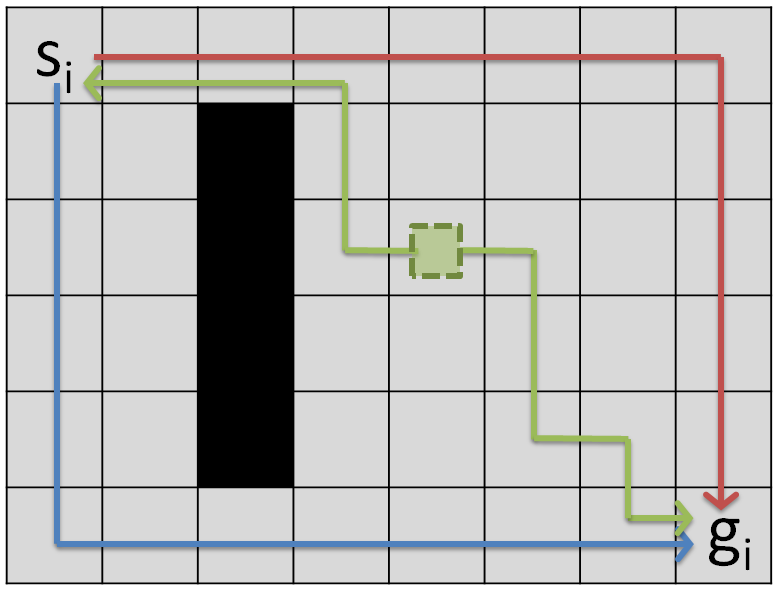
\includegraphics[width=0.45\columnwidth]{img/distant_ok.PNG}
\caption{By choosing a different starting location, the greedy algorithm finds a better green path than in Figure~\ref{fig:distant_wrong}. In this example there are multiple possible starting locations, each equally good. If this happens, one is chosen at random.}
\label{fig:distant_ok}
\end{subfigure}

\caption{An example showing the drawback of finding the shortest path greedily from the the starting location $s_i$. This issue can be fixed by choosing different starting vertex. The green path is chosen after red and blue paths.}
\label{fig:distant}
\end{figure*}

% \subsection{Single Path}
First, we use the same approach as in the original study~\cite{AAMAS_corridors}.
For each agent, we choose a single random shortest path. The restricted graph $Gres_{0}$ is induced by $SP_A = \bigcup_{a_i \in A} SP_i$. Recall that $SP_i$ are the vertices on the shortest path for agent $i$. We refer to this approach as \emph{single-path} or \pss{} for short.



% \subsection{All Paths}
The second approach is on the other end of the spectrum. Instead of just one shortest path, we will consider all vertices on all of the possible shortest paths of a given agent. Formally, we write $SP_i^{All} = \{ v \in V \: | \: dist(s_i,v) + dist(v,g_i) = |SP_i|\}$ meaning all vertices whose distance from start location plus the distance to goal location equals the distance of a shortest path. The restricted graph $Gres_{0}$ is induced by $SP_A^{All} = \bigcup_{a_i \in A} SP_i^{All}$.

Note that while there may be many different shortest paths as discussed in Figure~\ref{fig:diagonal_example}, the number of vertices on those paths is much smaller. For the creation of the restricted graph, we are interested only in the vertices, the specific path will be decided by the underlying solver. Finding all of the vertices on all of the shortest paths can be done by performing a breath-first search from the start and goal of the agent and checking for the condition in the definition of $SP_i^{All}$. We refer to this approach as \emph{all-paths} or \psa{} for short.




% \subsection{Random Paths}
%
Instead of considering one or all possible paths, we aim to pick vertices that are part of just some subset of all paths. First, we need to set a number of paths to consider. Note that based on the given map and the start and goal locations of each agent, there is a wide variety of the number of shortest paths. Instead of selecting a magic constant, we propose to find $\frac{|SP_i^{All}|}{|SP_i|}$ shortest paths for agent $a_i$ and consider the union of vertices on those. If there is a unique shortest path, by using the formula we correctly consider just the one shortest path, while on an empty $N \times N$ grid (such as in Figure~\ref{fig:diagonal_example}), we are considering $\frac{N}{2}$ paths.

The next proposed approach picks the specified number of shortest paths randomly. We do this by a random walk starting at $s_i$ moving only over vertices from $SP_i^{All}$ in the correct direction. We know the correct direction based on the distance from $s_i$ and $g_i$ computed by BFS (we need to perform the two BFS in order to determine $SP_i^{All}$). The random walk is biased to prefer vertices that are not yet used for a given agent. By doing this for all agents we get $SP_A^{Rand} = \bigcup_{a_i \in A} SP_i^{Rand}$. We refer to this approach as \emph{random-paths} or \psr{} for short.




% \subsection{Distant Paths}
%
The drawback of \emph{random-paths} it that there is no guarantee on the properties of the chosen shortest paths. The idea of using more than one shortest path is to allow the underlying solver to navigate the agent through a different region of the map to avoid possible conflicts. However, by choosing random paths, we may produce paths that share many vertices or are in close proximity to each other, both of which are undesirable.

We want to find \emph{diverse} and \emph{distant} paths. There is a polynomial-time algorithm to find diverse shortest paths~\cite{diverse}. In this case, diverse means paths that share the least amount of edges (or vertices). By using this algorithm, it may be the case that we find paths as shown in Figure~\ref{fig:diverse}. On the other hand, there is also a research dealing with finding the most diverse near-shortest paths~\cite{distant}, in which case the paths are supposed to be the greatest distance from each other. Note that both studies use the term distant with different meaning. In our paper we will be using \emph{diverse} for different paths and \emph{distant} for path with distance between them. The downside of the the second referred study is that the paths found are not optimal and also the problem itself is NP-Hard, which is not a desirable trait for a preprocessing function.

\begin{figure}[hb]
\centering
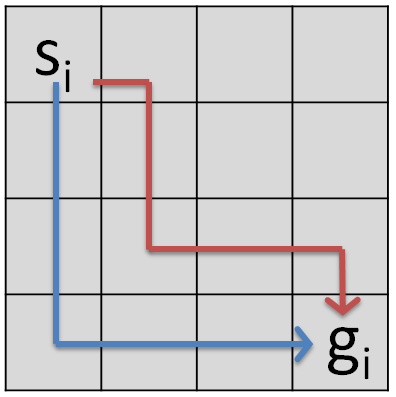
\includegraphics[width=0.25\columnwidth]{img/diverse.PNG}
\caption{Possible shortest paths from $s_i$ to $g_i$ found by using the diverse shortest paths algorithm~\cite{diverse}.}
\label{fig:diverse}
\end{figure}


Our proposed approach will be heuristic. Again, we build the paths over the vertices from $SP_i^{All}$, gradually creating $SP_i^{Dist}$. At each step, we try to add a new vertex to the currently build path and if there are multiple choices, we pick one that maximizes the minimal distance to all of the vertices currently in $SP_i^{Dist}$ (see Figure~\ref{fig:distant_choose} for an example).

\begin{figure}[ht]
\centering
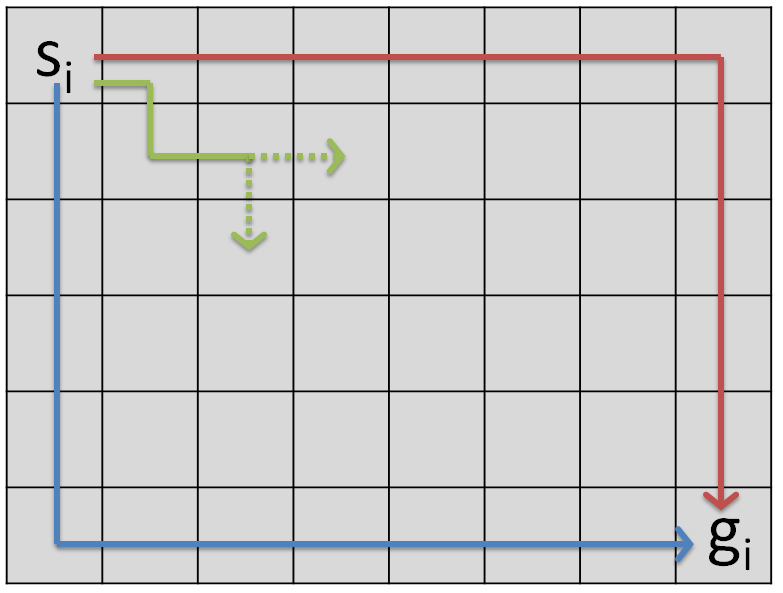
\includegraphics[width=0.45\columnwidth]{img/distant_choose.PNG}
\caption{The gradual building of $SP_i^{Dist}$ from $s_i$ to $g_i$ by a greedy approach. The currently build green path has a choice. Moving downward will be chosen since it maximizes the distance to the already chosen paths.}
\label{fig:distant_choose}
\end{figure}

Since this is just a heuristic, there are examples that make us choose an undesirable path because the approach greedily chose the next vertex on the path without knowledge of the rest of the map. Such example can be seen in Figure~\ref{fig:distant_wrong}. To mitigate this, we start to build the path from a different vertex from the set $SP_i^{All}$ rather than from $s_i$. The first path is build the same as $SP_i$, for the latter paths, we choose a vertex $v$ such that it maximizes the minimal distance to all of the vertices currently in $SP_i^{Dist}$. This way we need to build the path both from $v$ to $s_i$ and from $v$ to $g_i$. Using this approach we find a much more desirable path for the example in Figure~\ref{fig:distant_wrong} with the result shown in Figure~\ref{fig:distant_ok}. We will refer to this approach as \emph{distant-paths} or \psd{} for short.

%%% Local Variables:
%%% mode: latex
%%% TeX-master: "main"
%%% End:
